\documentclass[11pt]{article}

\usepackage{amsmath}
\usepackage{amssymb}
\usepackage{graphicx}
\usepackage{enumitem}
\usepackage{tikz}
\usetikzlibrary{positioning}
\usepackage[margin=1in]{geometry}
\usepackage[colorlinks=true, urlcolor=blue]{hyperref}

\graphicspath{{plots/}{../plots/}{./}}

\newcommand{\answer}{\par\noindent\textbf{Answer:} }
\newcommand{\todo}[1]{\textcolor{red}{\textbf{TODO:} #1}}

\title{AA274A Homework 4}
\author{Name: Colin Skinner\\ SUNet ID: 06525671}
\date{}

\begin{document}
\maketitle

\noindent\textbf{Collaborators:} None

\noindent\textbf{Use of generative AI:} LaTeX report formatting and debugging (GTSam due to syntax, and loop index issues)

%%%%%%%%%%%%%%%%%%%%%%%%%%%%%%%%%%%%%%%%%%%%%%%%
\newpage
\section*{Problem 1: Convolutions and Image Features}

\subsection*{(i)}
Graded by the autograder; nothing to include.

\subsection*{(ii)}
\begin{center}
    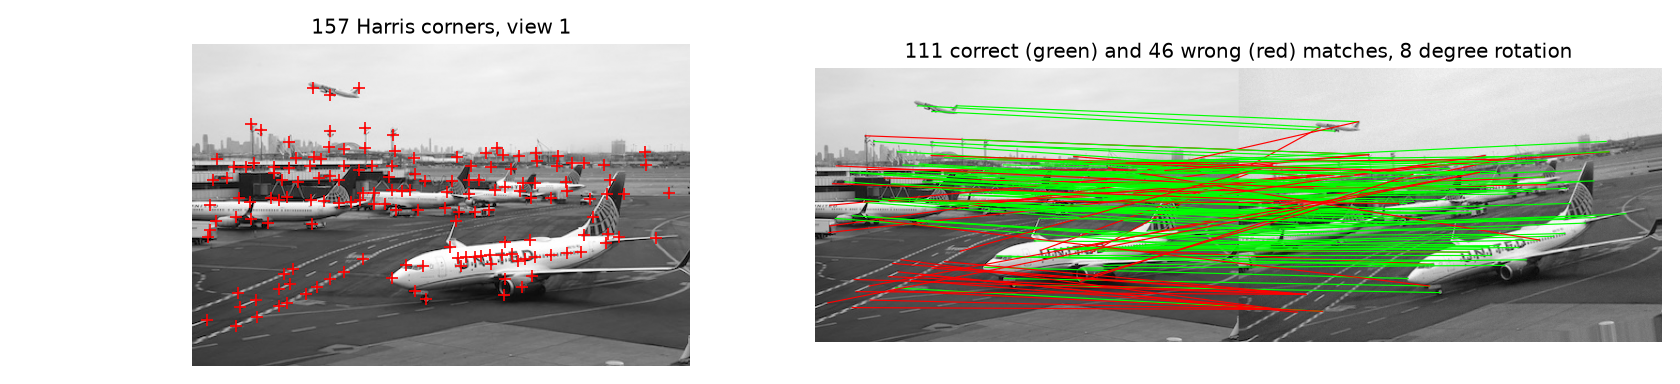
\includegraphics[width=\linewidth]{p1_matches.png}
\end{center}

\answer Corners in first view: 157; corners in second view: 144; correct matches: 111 (of 157)

Every point is linked to a match, which fails if a point is missing from the next image (since it just takes the argmax), or if there is a completely different point that happens to be a better match (e.g. repeated patterns such as the runway).

RANSAC could be used because it is robust to outliers, so if a vector is very wrong, the transformations using it as a basis will perform worse using the algorithm. Then the outliers can be removed from the best-fit transformation.

\subsection*{(iii)}
A flat region would have similar-looking windows along both directions, so not very distinctive. An edge constrains it to one dimension, but the windows are still similar-looking going up/down or left/right on the edge. A corner constrains that additional dimension.

\begin{center}
    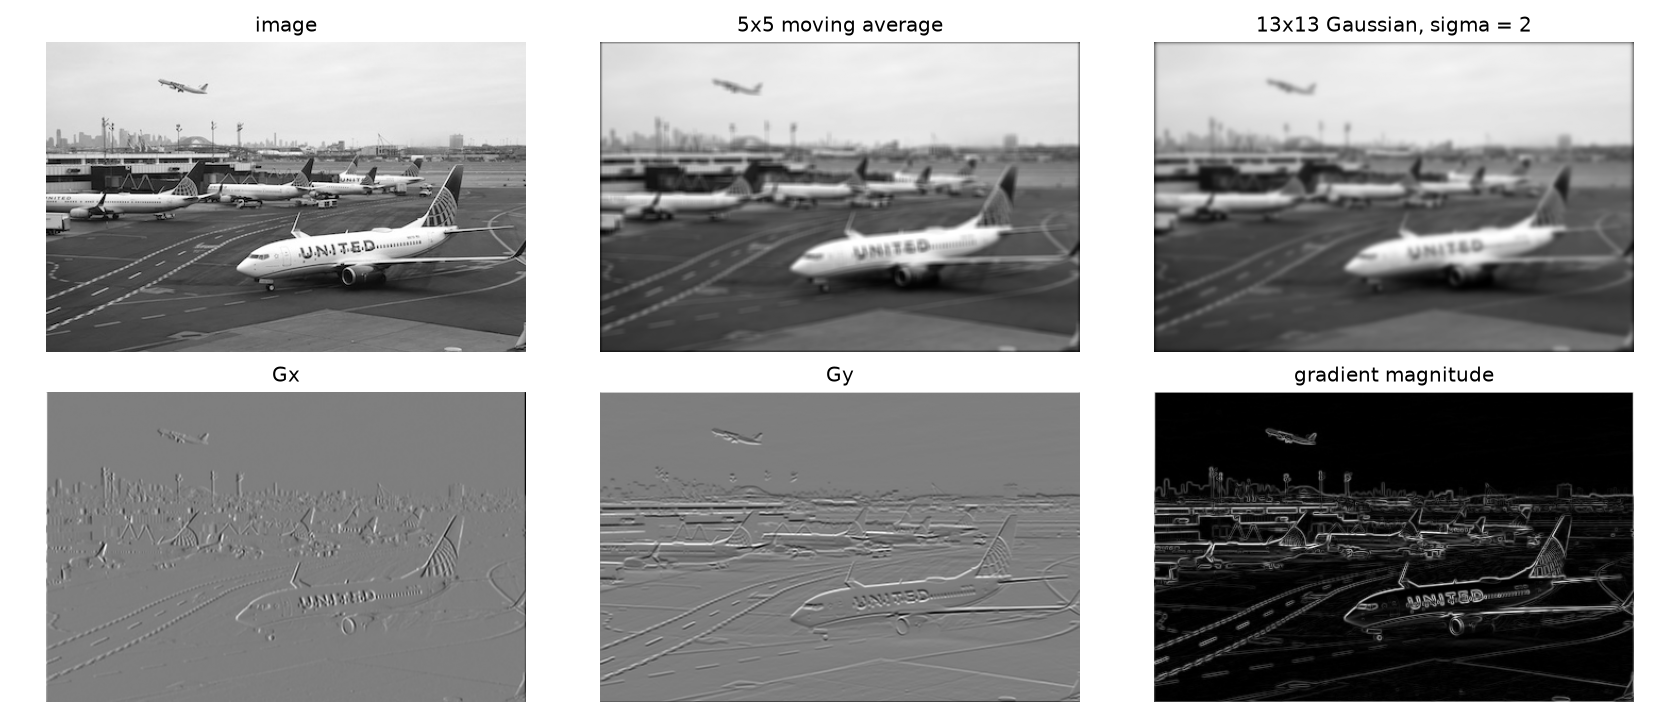
\includegraphics[width=\linewidth]{p1_filters.png}
\end{center}

The gradient magnitude has a bright border frame because of the zero padding. Therefore, when there are lighter pixels right next to the border, it gets detected as an edge (as it is in fact a large gradient). One fix could be extrapolating the edge pixels to the boundary.

\subsection*{(iv)}
\begin{center}
    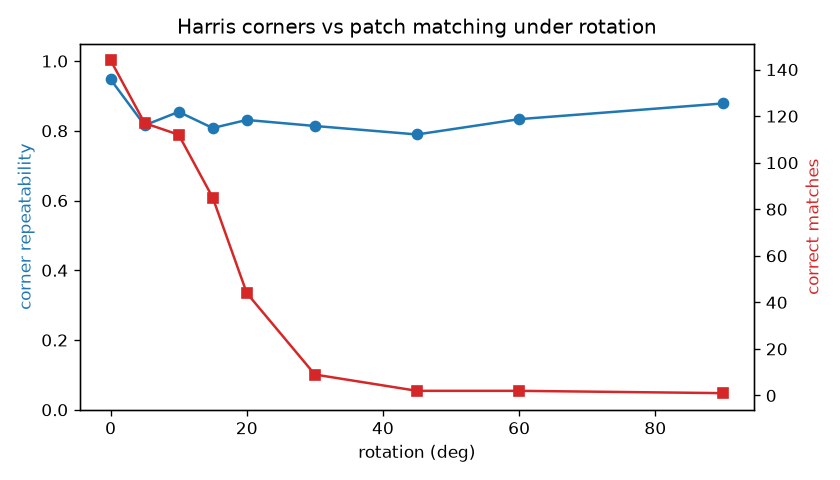
\includegraphics[width=0.6\linewidth]{p1_rotation.png}
\end{center}

\answer
\begin{center}
\begin{tabular}{c|c|c}
Rotation & Repeatability & Correct matches \\ \hline
$0^\circ$  & 0.947 & 144 of 157 \\
$30^\circ$ & 0.814 & 9 of 157 \\
$90^\circ$ & 0.879 & 1 of 157
\end{tabular}
\end{center}

Harris detector is good with corners because it only checks for strong gradients in multiple directions, but the patch detector is tied to the image's x and y grid. That is why repeatability is relatively good with corners being detected in both, across rotations.


\subsection*{(v)}
\noindent\textbf{(a)}

\answer Maximum difference away from the border: $4.35 \times 10^{-15}$


Associativity is useful because rather than having to repeatedly convolve kernels onto a larger image, the smaller kernels can be convolved with themselves, and only the final combined one will be applied onto the larger image. It may not be as useful if the kernels are close to the size of the image though.

\medskip
\noindent\textbf{(b)}

\answer Direct $13\times 13$ Gaussian: $13^2 = 169$ multiplications per pixel; separable: $13 + 13 = 26$ multiplications per pixel

\medskip
\noindent\textbf{(c)}

\answer Weights in one $3\times 3$ mask: $9$; receptive field after three $3\times 3$ convolutions: $7\times 7$; layers needed for a $15\times 15$ receptive field: $7$

Each $3\times 3$ layer grows the receptive field by $2$, so $L$ layers give $1 + 2L$ so evaluated, it is $1 + 2L = 15 \rightarrow L = 7$.

%%%%%%%%%%%%%%%%%%%%%%%%%%%%%%%%%%%%%%%%%%%%%%%%
\newpage
\section*{Problem 2: Bundle Adjustment SLAM with GTSAM}
\subsection*{(i)}

\begin{figure}[h!]
    \centering
    \includegraphics[width=0.6\linewidth]{factor_graph.png}
\end{figure}

\answer Number of factors (including the prior): $8$ (1 prior, 2 odometry, 4 range-bearing, 1 loop closure)

\subsection*{(ii)}
Graded by the autograder; nothing to include.

\subsection*{(iii)}
\begin{center}
    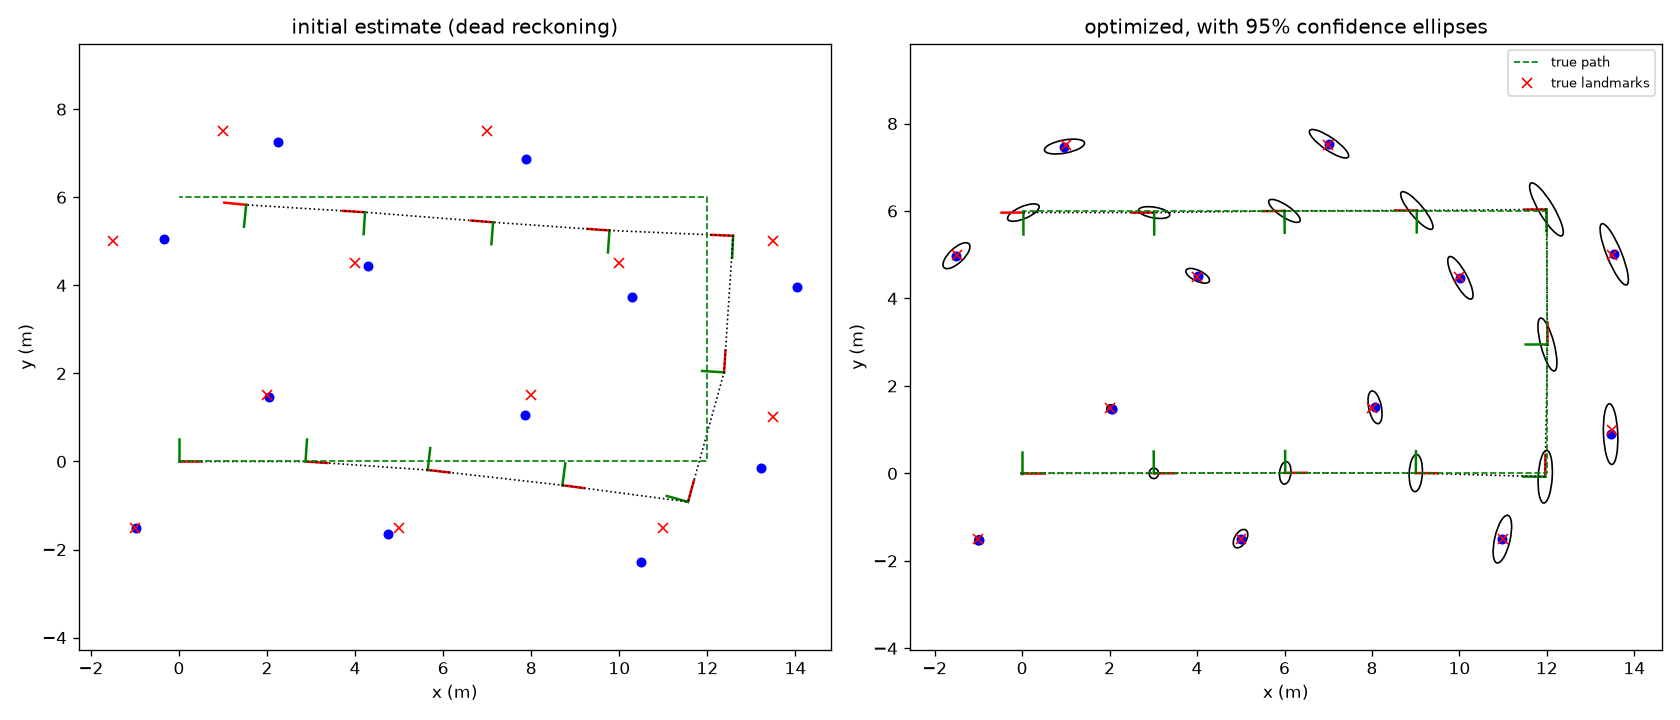
\includegraphics[width=\linewidth]{p2_slam_5.png}
\end{center}

\answer Total factors: 55; prior factors: 1; odometry factors: 10; range-bearing factors: 43; loop-closure factors: 1

\answer Maximum position error (dead reckoning): 1.536 m; maximum position error (optimized): 0.084 m

\subsection*{(iv)}

The pose ellipses grow as the robot travels because of drift, but shrink in the end because of being linked with loop closure, along with seeing landmarks that it has mapped out well from the start. 

The landmarks that have smaller ellipses are either seen from many poses (so have good connectivity), or are close to the start (which is close to the prior). Conversely, the landmarks with the largest ellipses are seen from few poses, or poses with large ellipses themselves (e.g. the ones on the very right are seen by poses with large ellipses themselves).

\subsection*{(v)}
\begin{center}
    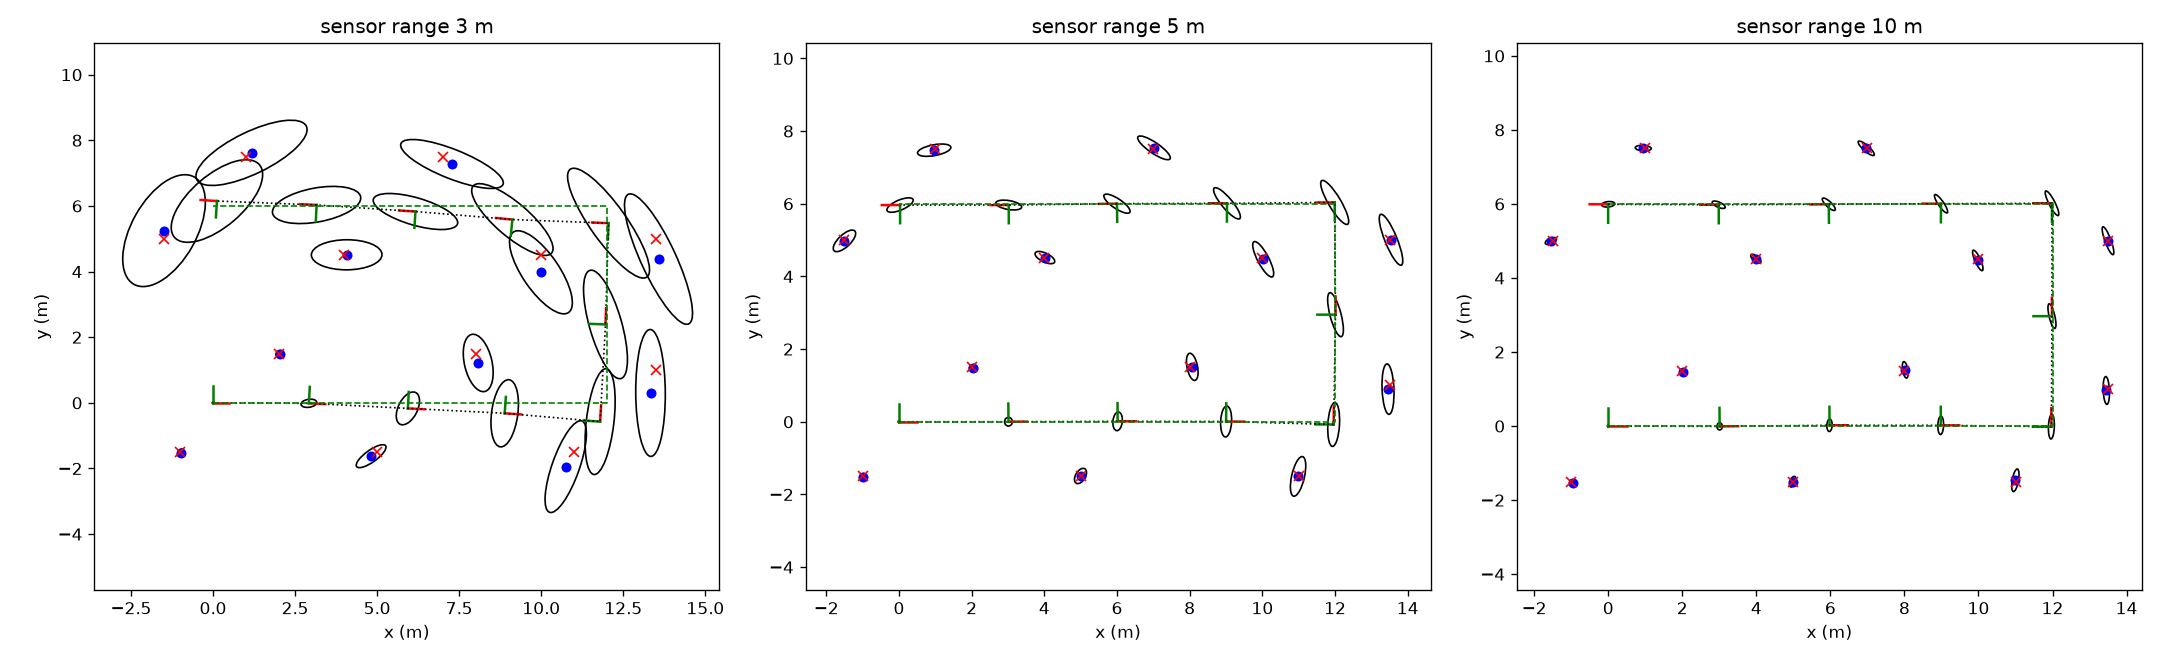
\includegraphics[width=\linewidth]{p2_ranges.png}
\end{center}

\answer
\begin{center}
\begin{tabular}{c|c|c}
Sensor range & Number of factors & Maximum position error (m) \\ \hline
$3$ m  & 35  & 0.612 \\
$5$ m  & 55  & 0.084 \\
$10$ m & 111 & 0.044
\end{tabular}
\end{center}

As explained, 10m range provides the robot with more range-bearing measurements, increasing the connectivity of the graph and decreasing uncertainty/error.

\answer
\begin{center}
\begin{tabular}{c|c|c}
Sensor range & Final-pose std.\ with loop closure (m) & Without loop closure (m) \\ \hline
$3$ m  & 0.767 & 1.379 \\
$5$ m  & 0.169 & 0.169 \\
$10$ m & 0.078 & 0.078
\end{tabular}
\end{center}

The 10m range allows the robot to have more graph connectivity with further landmarks. A 3m range does not have good connectivity, so adding loop closure to 3m will have a larger impact than the marginal improvement it adds as an additional connection for the 10m range.

\end{document}
